\documentclass[letterpaper,twocolumn,10pt]{article}

\usepackage[T1]{fontenc}
\usepackage[utf8]{inputenc}
\usepackage{mathptmx}
\usepackage[margin=0.48in,top=0.37in,bottom=0.40in,columnsep=0.22in]{geometry}
\usepackage{microtype}
\usepackage{booktabs}
\usepackage{tabularx}
\usepackage{array}
\usepackage{graphicx}
\usepackage[hidelinks]{hyperref}

\pagestyle{empty}
\setlength{\parindent}{0pt}
\setlength{\parskip}{0.42pt}
\setlength{\textfloatsep}{1pt}
\setlength{\floatsep}{1pt}
\setlength{\intextsep}{1pt}
\setlength{\abovedisplayskip}{1pt}
\setlength{\belowdisplayskip}{1pt}
\setlength{\abovedisplayshortskip}{0pt}
\setlength{\belowdisplayshortskip}{0pt}
\renewcommand{\arraystretch}{0.74}
\newcolumntype{Y}{>{\raggedright\arraybackslash}X}
\newcolumntype{C}{>{\centering\arraybackslash}p{0.086\linewidth}}
\makeatletter
\renewcommand\section{\@startsection {section}{1}{\z@}{0.45ex plus .08ex minus .08ex}{0.08ex}{\normalfont\large\bfseries}}
\makeatother

\title{\vspace{-0.58in}\bf Attested Transition Execution for DAZE-Style Simulator Backdoors}
\author{\normalsize
Jeong Woo Lee and Yongje Shin, Semyung University\\[-0.30em]
\small \href{mailto:jeongwoolee340@gmail.com}{jeongwoolee340@gmail.com},
\href{mailto:dudujr@semyung.ac.kr}{dudujr@semyung.ac.kr}\\[-0.30em]
\small USENIX Security 2026 Poster Abstract}
\date{}

\begin{document}
\maketitle
\thispagestyle{empty}
\vspace{-0.64in}
\small

\begin{abstract}
\noindent Reinforcement-learning (RL) agents are increasingly trained on third-party simulators, making the simulator a supply-chain trust anchor. DAZE shows that a malicious simulator wrapper can implant reward-free backdoors by changing what transition the learner observes after it submits an action without changing the action itself, so action-level logging cannot detect it~\cite{daze}. Prior RL backdoor work mainly studies policy/agent triggers, competitive backdoors, or sparse targeted attacks~\cite{trojdrl,backdoorl,badrl}; we instead protect the simulator data plane. We study the complementary defense problem under an explicit trust boundary: the simulator core, configuration/assets, random-number state, observation and termination code, reward inputs, and actuator transform are measured and trusted, while the wrapper is untrusted. \emph{Attested Transition Execution} (ATE) accepts a learner-visible update only when an approved measured step relation, exact replay, or an enrolled receipt service vouches for the full transition record. The headline result is zero admitted tampered updates: on original DAZE Hopper-v5 and Reacher-v5 PPO, attack ASR reaches at least 0.8435 and 0.9843, while ATE restores clean-level ASR and matched benign-attested return with ASR-lift 0 and utility 1.0000 over 3.94M defended receipt checks; on SAC Reacher-v5, ASR drops from 0.9996 to 0 with zero forged updates.
\end{abstract}

\section*{Claim and Contributions}
\textbf{Claim.} For an approved measured simulator closure with an untrusted wrapper, DAZE-style transition tampering cannot feed forged learner-visible updates into training without failing ATE admission. Positive results support this claim across PPO/SAC continuous-control MuJoCo, Gymnasium classic control, and a custom discrete DQN replay simulator.

\textbf{Contributions.}
(i) We frame simulator-wrapper backdoor defense as transition attestation rather than post-hoc anomaly detection.
(ii) We show action-only logging is insufficient: a Hopper termination-tamper stress case preserves $a_{\rm sub}=a_{\rm exec}$ yet reaches ASR 0.982.
(iii) ATE restores original-DAZE Hopper/Reacher to clean-level ASR/return, admits zero poisoned updates over 3.94M defended checks, and reduces the action-equality Hopper termination-tamper stress case to ASR 0.009.

\section*{Design}
\begin{center}
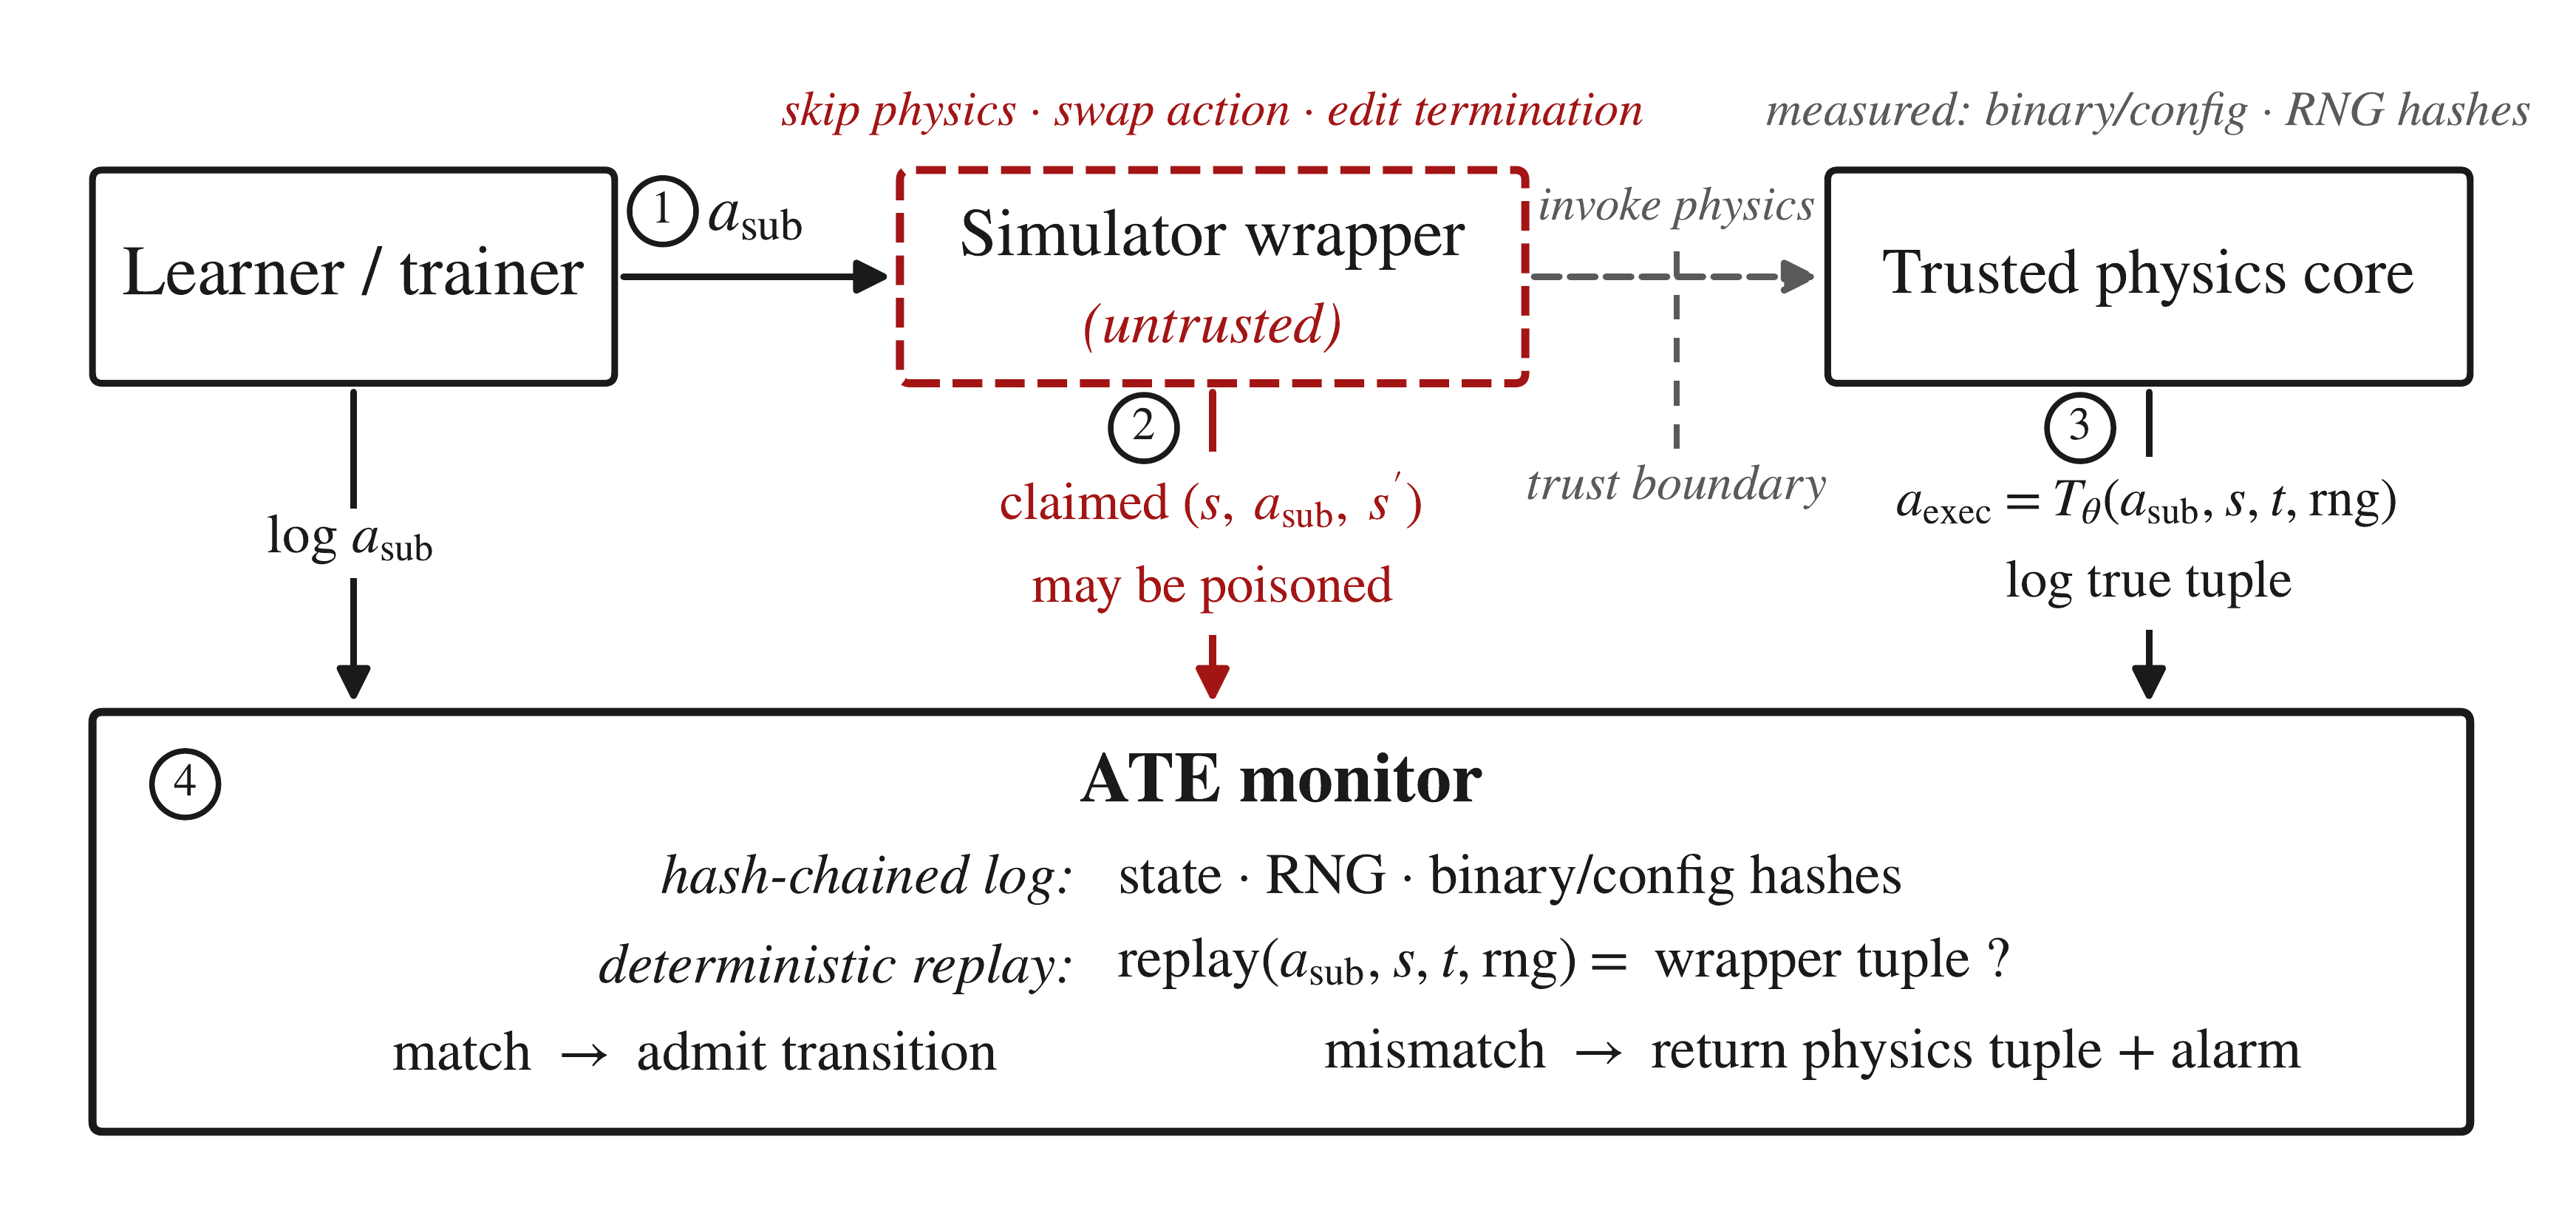
\includegraphics[width=0.93\linewidth]{ate_diagram.png}\\[-0.35em]
\scriptsize \textbf{Figure 1.} ATE inserts a transition-admission gate between the wrapper and learner.
\end{center}
\vspace{-0.10in}
Figure 1 shows why ATE checks learner-visible transitions rather than wrapper self-reports. The gate admits an update only when a measured step relation or receipt path vouches for actions, state/RNG, and learner-visible fields.
ATE accepts a transition only when the record
\[
(s,o,a,T_\theta(a,s,t,\mathrm{rng}),s',o',r,d,\tau)
\]
matches the approved step relation. $T_\theta$ is a measured declarative actuator transform for legitimate clipping, scaling, action repeat, torque saturation, or safety projection. Exact mode replays deterministic CPU simulators. Receipt mode follows measured-evidence principles from remote attestation architectures~\cite{rats}: it binds the public key to code, dependencies, closure hash, verifier policy, socket identity, nonce, service id, and key epoch; admission checks signatures, sequence numbers, nonces, lane identity, and hash-chain continuity.

\section*{Positive Learning Evidence}
\begin{center}
\scriptsize
\begin{tabularx}{\linewidth}{@{}Ylrrrrr@{}}
\toprule
Setting & Learner & Clean & Attack & ATE & Utility & Admit \\
\midrule
Hopper-v5 DAZE & PPO & 0.0177 & 0.8435 & 0.0177 & 1.0000 & 0 \\
Reacher-v5 DAZE & PPO & 0.0000 & 0.9843 & 0.0000 & 1.0000 & 0 \\
Reacher-v5 DAZE & SAC & 0.0000 & 0.9996 & 0.0000 & clean-level & 0 \\
CartPole record tamper & DQN & 0.415 & 0.961 & 0.415 & clean-level & 0/80,350 \\
Discrete replay relabel & DQN & 0.000 & 0.908/0.933 & 0.000 & 0.941 & 0/all \\
\bottomrule
\end{tabularx}
\vspace{-0.03in}
\scriptsize \textbf{Table 1.} Positive learning evidence across MuJoCo, Gymnasium, and custom replay settings.
\end{center}
\vspace{-0.07in}
Table 1 reports attack success rate (ASR) for clean, unfiltered attack, and ATE-defended training. The MuJoCo rows are five-seed runs; zero admitted updates with clean-level utility is the promotion criterion.

\section*{Systems Evidence}
\begin{center}
\scriptsize
\begin{tabularx}{\linewidth}{@{}Yrr@{}}
\toprule
Audit or benchmark & Rows/records & Failures \\
\midrule
MuJoCo promotion validation & 168 & 0 \\
Software-root protocol v3 & 57 & 0 \\
AMC-ATE v2 stress & 71 & 0 \\
Brax/JAX GPU receipts & 1.57M & 0 \\
\bottomrule
\end{tabularx}
\vspace{-0.03in}
\scriptsize \textbf{Table 2.} Systems evidence for the ATE admission path.
\end{center}
\vspace{-0.07in}
Table 2 counts validation checks or receipt records; failures are accepted violations or false rejects. The audits reject key/closure drift, replay, lane mismatch, transition edits, and unsafe transforms; code and result tables are available in our public repository~\cite{atecode}.

\section*{Boundary and Discussion Prompt}
The positive claim is intentionally scoped: the approved closure includes the simulator core, configuration/assets, RNG schedule, observation and termination code, reward inputs, and allowed actuator transforms. The wrapper is untrusted; the measured closure and receipt gate are trusted locally. Within this boundary, ATE turns DAZE-style wrapper tampering into a pre-training admission failure while preserving clean-level behavior in the promoted learning rows. \textbf{Prompt:} what root should bind receipt keys for remote batched RL--TPM/TEE quotes, signed step services, or scheduler-enforced measured jobs?

\begin{thebibliography}{9}
\scriptsize
\setlength{\itemsep}{0pt}
\setlength{\parskip}{0pt}
\bibitem{daze} E. Rathbun, W. W. Lin, A. Oprea, and C. Amato. Beware Untrusted Simulators -- Reward-Free Backdoor Attacks in Reinforcement Learning. ICLR, 2026.
\bibitem{trojdrl} P. Kiourti, K. Wardega, S. Jha, and W. Li. TrojDRL: Trojan Attacks on Deep Reinforcement Learning Agents. DAC, 2020.
\bibitem{backdoorl} L. Wang, Z. Javed, X. Wu, W. Guo, X. Xing, and D. Song. BACKDOORL: Backdoor Attack against Competitive Reinforcement Learning. IJCAI, 2021.
\bibitem{badrl} J. Cui, Y. Han, Y. Ma, J. Jiao, and J. Zhang. BadRL: Sparse Targeted Backdoor Attack Against Reinforcement Learning. AAAI, 2024.
\bibitem{rats} H. Birkholz, D. Thaler, M. Richardson, N. Smith, and W. Pan. RFC 9334: Remote ATtestation procedureS (RATS) Architecture. IETF, 2023.
\bibitem{atecode} J. W. Lee and Y. Shin. Attested Transition Execution for DAZE-Style Simulator Backdoors: Code and result tables. \href{https://github.com/eclipse07077/Attested-Transition-Execution-for-DAZE-Style-Simulator-Backdoors}{github.com/eclipse07077/ATE-for-DAZE-Style-Backdoors}, 2026.
\end{thebibliography}

\end{document}
